%!TEX root = ../thesis.tex

%%% Thesis Introduction --------------------------------------------------
\chapter{Introduction}

\graphicspath{ {Introduction/IntroductionFigs/PNG/}
  {Introduction/IntroductionFigs/PDF/}
  {Introduction/IntroductionFigs/} }

La modélisation géométrique a permis, dans un premier temps, de représenter des
objets virtuels. Ces objets peuvent être de natures différentes, comme les
surface paramétriques ou les maillages. Pour notre part, nous nous sommes
intéressés aux maillages, qui représente une discrétisation de l'espace sous
forme de cellules (sommets, arêtes, faces, volumes). Une méthode déformation
naïve consiste à déplacer des sommets d'un maillage. Mais d'autres types de
déformations, plus élaborés, se sont instaurés. Ils sont pour la plupart propres
à une représentation spécifique d'un maillage, mais d'autres, comme la
déformation \textit{spatiale}, font abstraction de ces représentations. Nous
nous sommes intéressés à ce type de déformation. Durant le reste du rapport,
nous appellerons \textit{objet} un maillage auquel nous appliquons une
déformation.\\
	
La déformation spatiale consiste à déformer un objet en modifiant son espace
ambiant au travers de la modification d'un outil. Cet outil est un objet et les
modifications qu'on peut lui appliquer sont réalisées au travers du déplacement
de ses sommets. Cet outil a des caractéristiques spécifiques, comme sa dimension
(point, courbe, surface, volume), la zone de l'espace qu'il déforme (limitée
spatialement ou globale) et sa résolution (nombre de sommets). On notera
\cite{Bar84} et \cite{SP86} comme étant les premiers à avoir introduit ce type
de déformation. L'avantage de ce procédé, par rapport aux méthodes déjà
existantes, a été de pouvoir réaliser des déformations indépendantes de la
représentation interne de l'objet à déformer.

\newpage

En pratique, la déformation d'un objet se décompose en 3 étapes :
\begin{enumerate}  

\item Construction de l'outil permettant la déformation

\item Association des points de l'espace composant l'objet à l'outil
(\textit{temps d'association})

\item Déformation de l'objet par invariance de l'association (\textit{temps de
déformation})

\end{enumerate} 

Les deux premières étapes ne sont réalisées qu'une seule fois. A la fin du temps
d'association, la dernière étape est réalisée à chaque manipulation de l'outil
de déformation. \\

Ce travail s'inscrit dans une démarche de création d'un nouvel outil de
déformation. Actuellement, pour déformer un objet, les artistes utilisent un
seul outil à la fois. Mais les différentes déformations ne peuvent pas toutes
être réalisées à l'aide des mêmes outils. Cette contrainte force les artistes à
recréer un nouvel outil lorsque la déformation qu'ils souhaitent appliquer n'est
pas possible. Cette étape est une tâche qui peut s'avérer longue. En effet il
est nécessaire de placer les différents points de contrôle de l'outil autour de
l'objet à déformer, et en fonction de la déformation voulue, leur nombre peut
devenir très important. Ce nombre de points de contrôle peut rendre le temps
d'association de l'outil assez important, même si cette étape n'est normalement
réalisée qu'une seule fois. L'idée serait alors d'avoir un \textit{multi-outil}
composé de plusieurs \textit{sous-outils} communiquant ensemble et déformant
chacun différentes zones de l'objet. Aussi, il serait agréable de pouvoir
générer automatiquement un multi-outil en fonction des caractéristiques de
l'objet à déformer, afin de simplifier au maximum le travail des artistes. Dans
la suite de ce travail, nous appelerons \textit{outil multidimensionnel}, un
multi-outil composé de plusieurs sous-outils de dimensions différents.

Considérons que notre objet soit un alligator (Figure \ref{INTall}), on souhaite
ouvrir la bouche de l'alligator, élargir son ventre et bouger sa queue, mais ces
déformations sont difficilement réalisables avec un seul outil. Pour obtenir le
comportement décrit plus-haut, une bonne proposition serait de créer d'associer
des axes pour la bouche, une cage pour le ventre et des points pour la queue. On
se demande alors comment mélanger les effets de ces outils de façon à ce que la
fonction résultant du mélange soit dérivable ($C^1$) et que l'aspect de la
déformation soit lisse. De plus, il semblerait intuitif d'associer à un outil
une zone d'influence limitée. Toujours en considérant notre alligator, lors de
l'ouverture de la bouche, on souhaiterait que le reste du corps ne soit pas
déformé par le déplacement des sommets de l'outil axial. \\

\begin{figure}[h]
  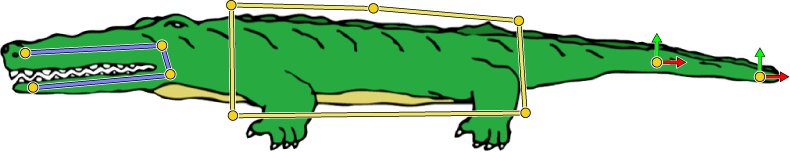
\includegraphics[scale=0.25]{alligator-avant}
  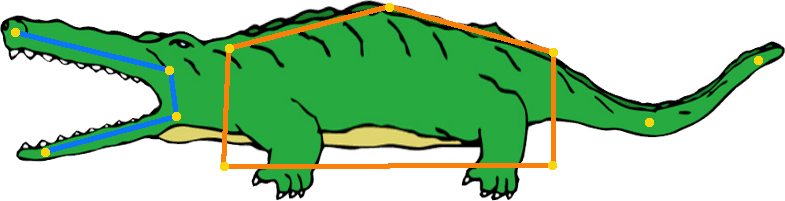
\includegraphics[scale=0.25]{alligator-apres}
  \caption{A gauche l'objet d'origine et à droite le même objet après
    déplacement de certains points de contrôle}
  \label{INTall}
\end{figure}

Nous avons travaillé sur la création d'un multi-outil de déformation. Nous nous
sommes concentré sur la création d'un multi-outil composé de plusieurs outils de
dimension 2 (faces).

La finesse d'une déformation est dépendante du nombre de degrés de liberté de
l'outil, mais de même, la complexité en temps de calcul de l'association de
l'outil à l'objet en est aussi dépendante. Partant de ce principe là, il
serait intéressant de disposer de plusieurs niveaux de résolutions d'un même
outil, afin de pouvoir choisir le niveau de résolution le plus adapté à la
déformation à appliquer. Mais cela implique la mise en place d'un moyen de
communication entre les différents niveaux de résolution, comme le modèle
proposé par \cite{Hur12} concernant les déformation de cages hiérarchiques. \\

Tout au long de ce travail, nos contraintes sont de fournir un outil
permettant de déformer des points de l'espace de manière interactive
et fluide, ainsi que d'obtenir des formulations mathématiques simples
et claires.
%%% ----------------------------------------------------------------------


%%% Local Variables: 
%%% mode: latex
%%% LaTeX-command: "latex -shell-escape"
%%% TeX-master: "../thesis"
%%% End: 
